\chapter{A practical approach of the finite element method}
\label{chap3}
\begin{shortAbstract}
The previous chapter explained in details how physics of anatomical structures could be described by continuun mechanics. When an organ is submitted to a force, the first effect of this application is a change in the organ's shape. This deformation can be measured using different strain tensors. By modelling the mechanical aspects of the material with an appropriate constitutive law, we can then deduce the stress tensor (or internal forces) at each point within the organ. The next step is to apply Newton's second law (law of conservation of momentum), which yields a partial differential equation at every point of the volume. The finite element method is a numerical procedure that allows to turn an infinite number of partial differential equations into a finite number of algebraic equations. The method follows different steps. We will first begin by describing the subdivision of the domain into smaller sub-domains into which local simpler equations are derived. We will then discuss how all the local equations are summed over the whole domain which eventually leads to the global solution. 
\end{shortAbstract}


\section{Introduction}

	\subsection{A numerical method}
One of the most important things engineers and scientists do is to model physical phenomena. Using assumptions concerning how the phenomena works and using the appropriate laws of physics governing the process, they can derive a mathematical model, often characterised by complex differential or integral equations relating various quantities of interest. However, because of the complexities in the geometry and complex boundary conditions found in real life problems, they cannot analytically solve these equations. A few decades ago, the only possible approach was to drastically simplify them, which was not always sufficient to find an approximate solution. Nowadays, in practice, most of the problems are solved using numerical methods. Indeed, with suitable mathematical models and numerical methods, computers can help solving many practical problems of engineering. Numerical methods typically transform differential equations governing a continuum to a set of algebraic equations of a discrete model of the continuum that are to be solved using computers \citep{Reddy93}. The \emph{finite element method} (FEM) is the most popular numerical procedure that is used to approximately solve differential equations, especially in continuum mechanics. 
	
	\subsection{The basic ideas of FEM}
The finite element method begins by dividing the structure into small pieces, manageable regions, called \emph{elements}. The collection of all these elements makes up a \emph{mesh} which approximates the problem geometry. Why is this a good idea? If we can expect the solution for an engineering problem to be very complex, it is mostly due to the complex geometry, on which a global solution is difficult to figure out. If the problem domain can be divided (\emph{meshed}) into small elements, the solution within an element is easier to approximate \citep{MacDonald07}. Over each finite element, the unknown variables are approximated using known functions. These functions can be linear or higher-order polynomial expressions that depend on the geometrical locations (\emph{nodes}) used to define the finite element shape. The governing equations are integrated over each finite element using linear algebra techniques and the solution over the entire domain problem is obtained by summing (\emph{assembling}) the solution of each element. Thus, the finite element method transforms an infinite number of differential equations (one can be defined at any point of the continuum) into a finite number of algebraic equations (depending on the chosen number of elements). 

This approach may be compared to trying to find the area under a curve. We know that we can find the exact solution for the area under the curve by integration. However, sometimes the function describing the curve is not known, or is difficult to integrate. One method to obtain an approximate solution is to break up the area into a series of rectangles and add the areas of all rectangles (see \fig{chap3:fig-areaUnderCurve}). It is worth nothing that the solution accuracy can be increased by reducing the width of the rectangles to better follow the curve. 
%
\begin{figure}[h]
\begin{center}
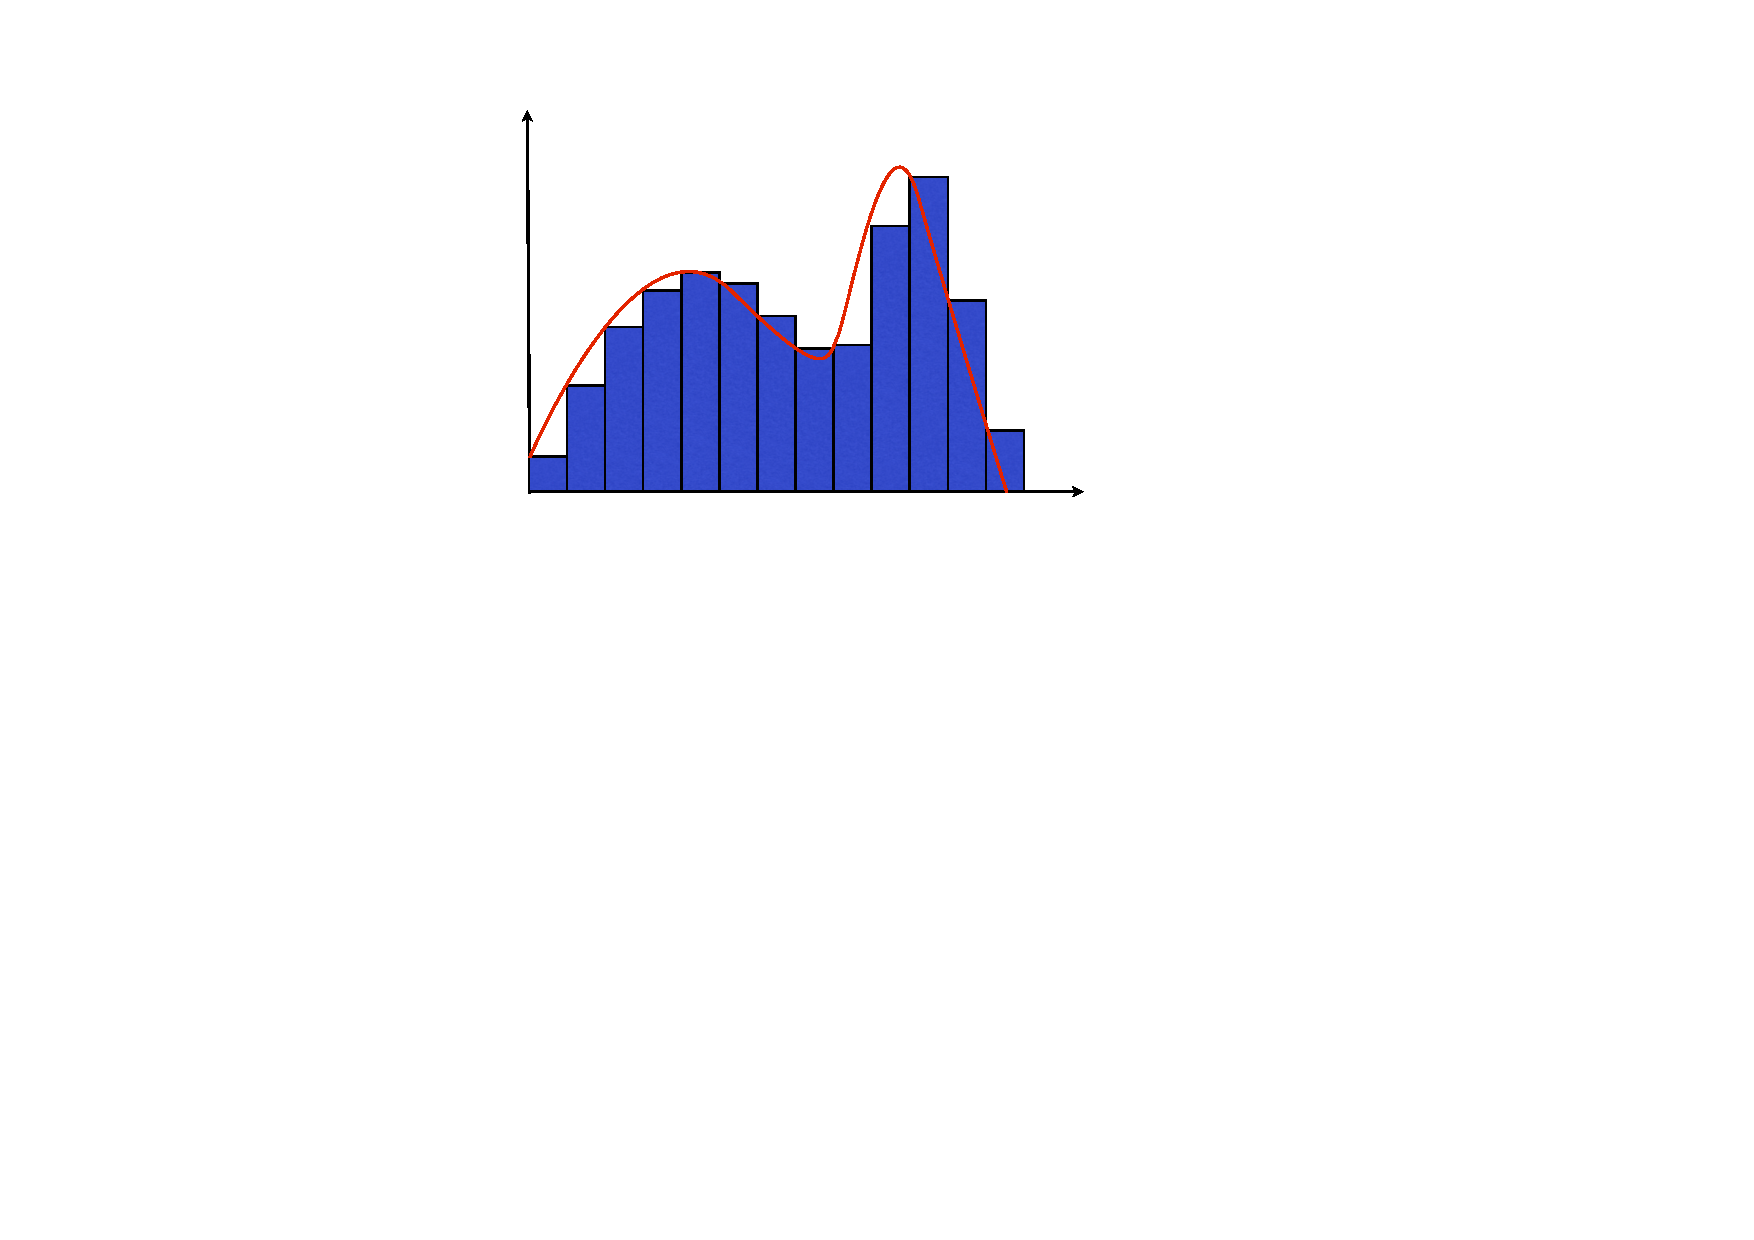
\includegraphics[width=8cm]{chapter3/areaUnderCurve.pdf}
\end{center}
\caption[Approximation of the area under a curve]{Approximation of the area under a curve by adding the areas of all rectangles (left Rieman sum for this example).}
\label{chap3:fig-areaUnderCurve}
\end{figure}

It is crucial to keep in mind that approximations occur at different stages during finite element analysis. The division of the whole domain into finite elements may not be exact (see \fig{chap3:fig-errorWithSubdivision}), introducing error in the domain being modelled. The second stage is when element equations are derived. As mentionned earlier, the unknowns of the problem are approximated using the idea that any continuous function can be representated by a linear combination of known functions and undetermined coefficients. Algebraic relations between the undetermined coefficients are then obtained by satisfying the governing equations over each element. There are a few types of approach for establishing these equations but, without going into details, the mathematical foundations of all these approaches are energy principles or the \emph{weighted residual methods} (see Appendix~\ref{appendix2}), which both lead to integrals during the process. Therefore, the second stage creates two sources of error: the representation of the solution by a linear combination of functions and the evaluation of the integrals. Finally, errors are introduced when solving the assembled system of algebraic equations. 
%
\begin{figure}[h]
\begin{center}
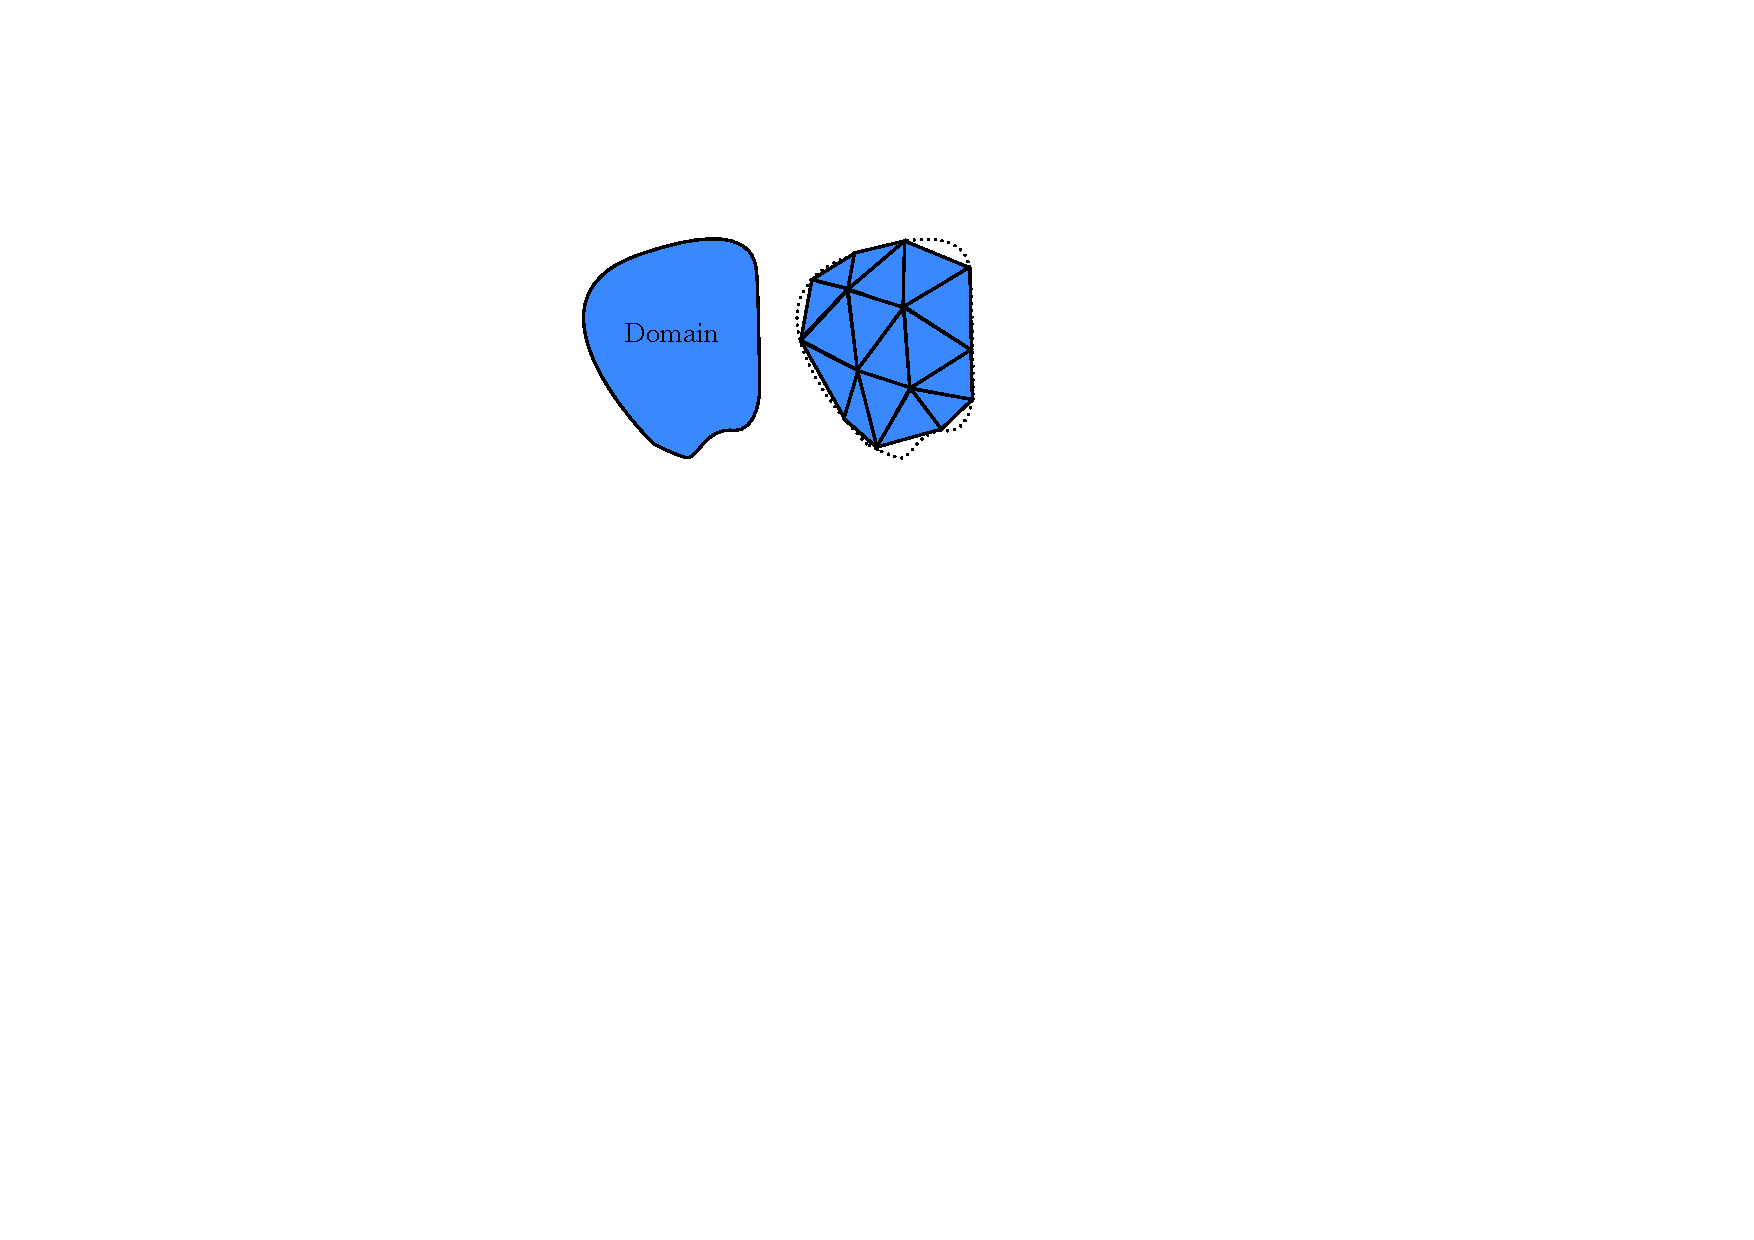
\includegraphics[width=8cm]{chapter3/errorWithSubdivision.pdf}
\end{center}
\caption[Error introduced by the division into elements]{The division of the domain into elements is not always perfect.}
\label{chap3:fig-errorWithSubdivision}
\end{figure}

\section{Discretisation}

	\subsection{Meshing process}
The first step in the finite element method is to create a mesh of the domain to study. Mesh generation is a very important task and can be very time consuming. The domain has to be meshed properly into elements of specific shapes. All the elements together form the entire domain of the problem without any gap or overlapping. For example, triangles or quadrilaterals can be used in two dimensions, and tetrahedra and hexahedra in three dimensions. Information, such as \emph{element connectivity}, must be created during the meshing process for later use in the formulation of the FEM equations. The number of elements into which the domain is divided in a problem depends mainly on the geometry of the domain and on the desired accuracy of the solution. Usually, the number of elements increases with the complexity of the geometry. For instance, if one part of the domain is thiner (see \fig{chap3:fig-sizeOfElementMeshing}), the size of the elements must be reduced in order to tile this particular part, which increases the total number of elements, and hence  the number of algebraic equations to solve. However, adding elements is sometimes desirable. Indeed, increasing the number of elements tends to get an approximate solution closer to the exact analytical solution (as reducing the width of the rectangles allows for a better approximation of the area under the curve). Elements are classically added in the particular regions of interest for a given problem, if this information is known a priori. A trade-off between accuracy and computational time must be found. This is why the meshing process on the problem domain must be carried out carefully. One needs to create a mesh which gives an accurate enough solution for the desired application while restraining the computational time according to the time constraints of the problem. As an example, finding the maximum load that can sustain a bridge in structural mechanics demands a high degree of accuracy, no matter how much time it is needed to compute the solution. Conversely, organ deformation in medical training simulators must be computed at an interactive rate so that no apparent delay can be observed between the manipulation of a given organ and its deformation. It does not mean that precision is not required, simply that the time constraints will necessarily limit the accuracy of the solution. 
%
\begin{figure}[h]
\begin{center}
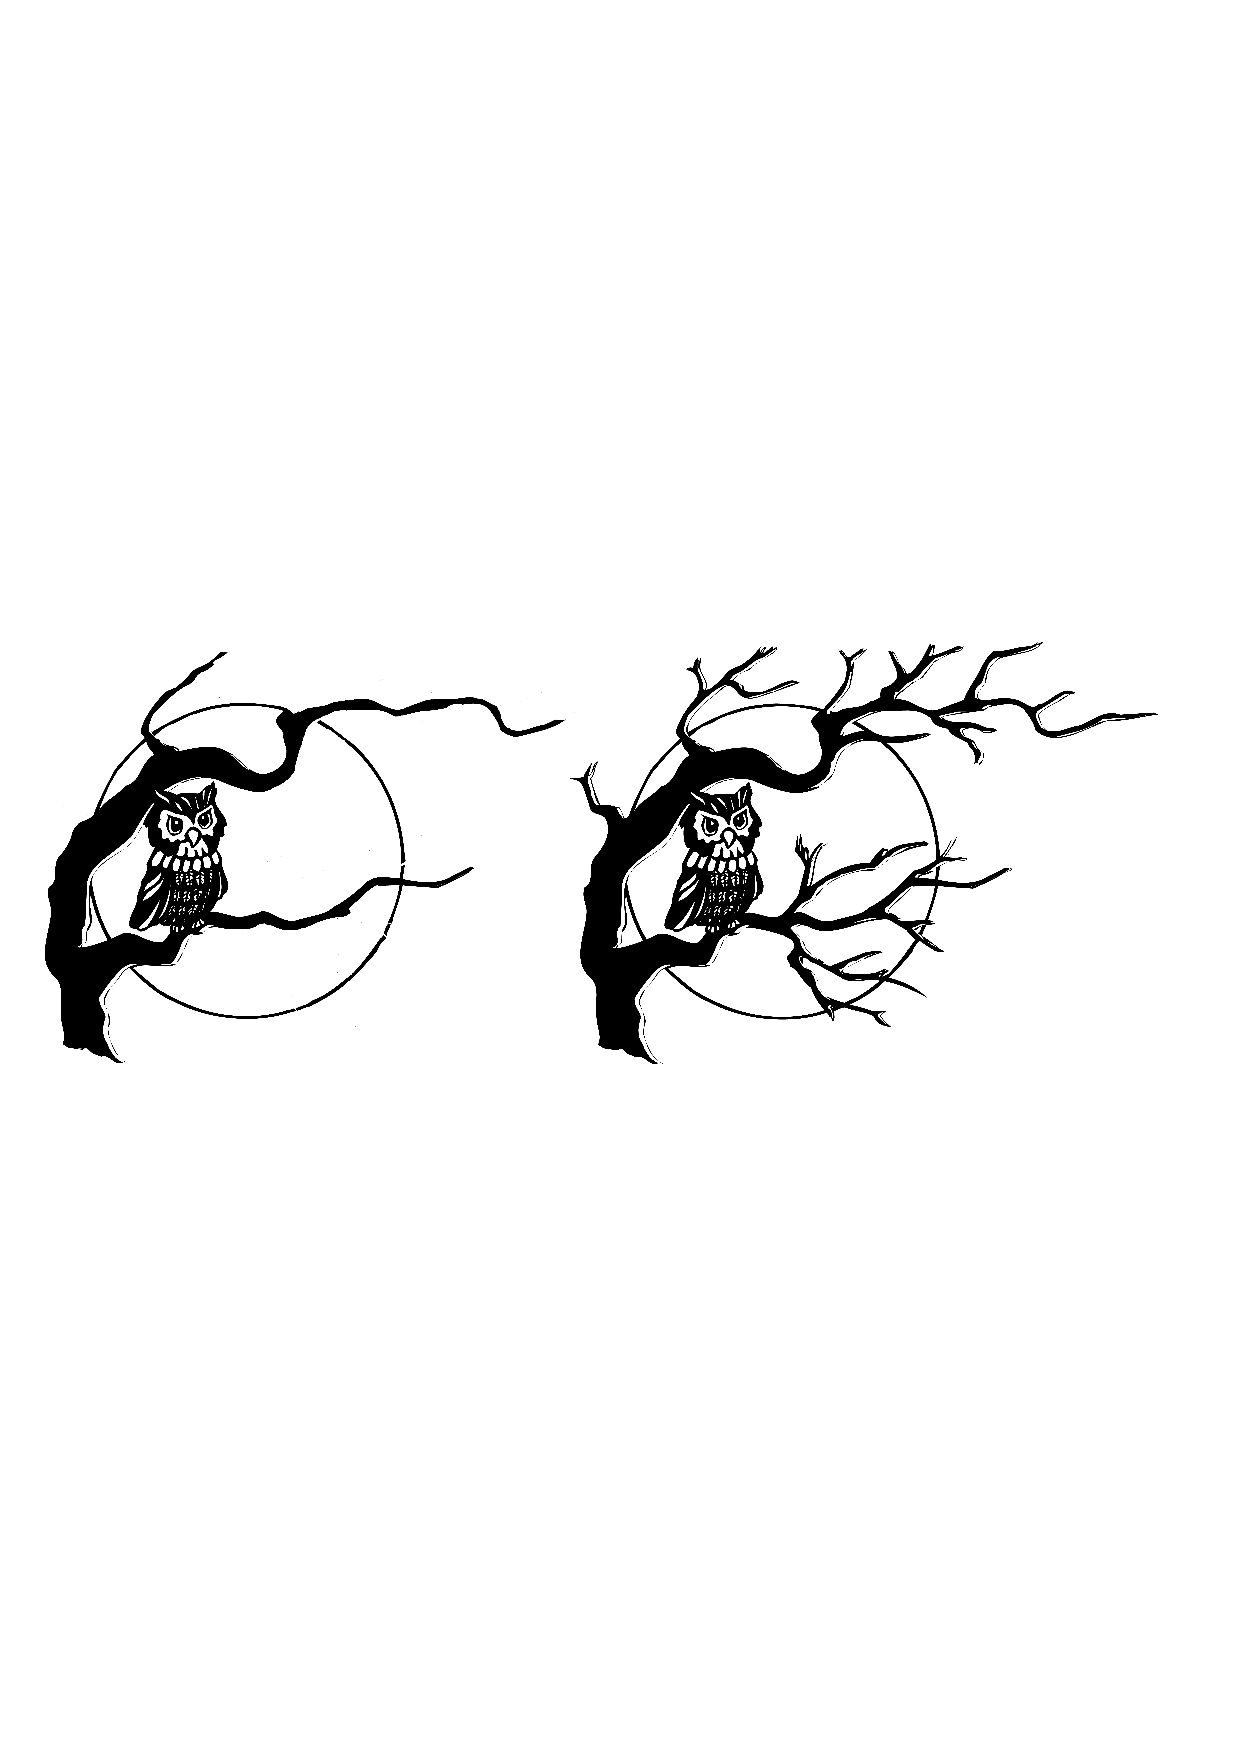
\includegraphics[width=13cm]{chapter3/sizeOfElementMeshing.pdf}
\end{center}
\caption[Finer mesh required for complex geometry]{By adding details on the tree's geometry \textbf{(right)}, the surface delimited by the tree becomes more difficult to mesh and would require smaller elements to tile all additional small branches.}
\label{chap3:fig-sizeOfElementMeshing}
\end{figure}


	
	\subsection{Solution interpolation}	\label{chap3:solutionInterpolation}
As we have seen, the finite element method is based on finding an approximate solution over each simple element rather than the whole domain. Any continuous function $ f $ may be approximated by a linear combination of known functions $ \phi_i $ and undetermined coefficients $ c_i $:
\begin{equation}
f \approx \tilde{f} = \sum_{i=1}^n c_i \phi_i .
\end{equation}
Moreover, the approximation solution $ u^e $within the element $\Omega_e $ must fullfill certain conditions of continuity in order to be convergent to the actual solution $ u $ as the number of elements is increased. The finite element method approximates the solution by the following polynomial expression:
\begin{equation}
\label{chap3:polynom}
u^e(x) = \sum_{i=1}^n u^e_i \psi^e_i(x) 
\end{equation}
where $ \Omega_e $ is a one-dimensional element\footnote{For the sake of simplicity, all derivations are carried out in 1D but remain valid for each component in higher dimensions.}, $ x $ a position within this element, $ u^e_i $ are the values of the solution $ u $ at the nodes and $ \psi^e_i(x) $ the approximation functions over the element. This particular form will be assumed for brevity but the interested reader may refer to \cite{Reddy93} for demonstration. Note that $ u^e_i  $ plays the role of the undetermined coefficients and $ \psi^e_i $ the role of approximation functions. Writing the approximation in terms of the nodal values of the solution is necessitated by the fact that we require the solution to be the same at points common to the elements in order to connect the approximate solution from each element and form a continuous solution over the whole domain. The approximation $ \psi^e_i $ can be linear or higher-order polynomial expressions and are called interpolation functions. 
%They are also commonly named \emph{shape functions} because they define the `shape' that a variable can take within an element (linear, quadratic etc.). 
Depending on the degree of polynomial approximation used to represent the solution, additional nodes may be identified inside the element. It is worth noting that the type of interpolation directly affects the accuracy of the solution. In other words, finding the solution to the problem consists of merely figuring out the values of the sought variable at every node of the mesh. Its value at any other point of the domain may then be deducted by interpolation within elements. 

\bigskip

The next logical question is how to derive the interpolation functions $ \psi^e_i  $ for a given element. Their derivation depends only on the geometry of the element and the number and location of the nodes. The number of nodes must be equal to the number of terms in the polynomial expansion. Therefore each element contains a single interpolation function for each of its nodes. As stated by interpolation theory, each interpolation function is required to be equal to $1$ at its corresponding node, and $0$ at all other nodes:
\begin{equation} 
	\psi^e_i(x_j) = \delta_{ij} = 
	\begin{cases} 
		1 & \text{if } i = j \\ 
		0 & \text{if } i \neq j
	\end{cases}
\end{equation}
where $ x_j $ is the position of node $j$. From there, we can state that the interpolation function at node $ i $ may be written as:
\begin{equation}
\psi^e_i(x) = C_i \prod_{i \neq j}^{n-1} (x-x_j)
\end{equation}
where $ j $ are the indices of the other nodes and $ C_i $ is a constant to be determined such as:
\begin{equation}
\psi^e_i(x_i) = 1.
\end{equation}
This function is zero at all nodes except the $i^{th}$ node. It is worth noting that such a definition for the interpolation functions $ \psi^e_i $ used in \eqref{chap3:polynom} yields:
\begin{equation}
u^e(x_j) = \sum_{i=1}^n u^e_i \psi^e_i(x_j) = u^e_j
\end{equation}
as expected. 

Since elements over the whole domain are generally not identical (different shapes), this process of determining all interpolation functions can become fastidious. We will now introduce a general method for defining interpolation functions which allows for arbitrary element shapes (subject to a given topology). To this end, we discuss the concept of element \emph{natural coordinates}.

	\subsection{Natural coordinates}
The natural coordinate system allows us to map every element into a typical and simpler element. As an example, an 8-node hexahedron element is shown in \fig{chap3:fig-naturalCoordinatesHexa} as it appears in the global $(x_1, x_2, x_3)$ and natural $(\xi_1,\xi_2,\xi_3)$ coordinate systems. While in its natural coordinate system the element is a regular aligned cube, in the global coordinate system the element may assume any admissible arbitrary form. Essentially, admissible means that the element must not be too distorted, and must certainly not fold back on itself. Another example is given \fig{chap3:fig-naturalCoordinatesTetra} with a tetrahedral element. The components of each node has a simple expression in natural coordinates, usually $0, 1$ or $-1$ and the centre of the coordinate system is taken at one of the nodes or at the centre of the element. 
%
\begin{figure}[h]
\begin{center}
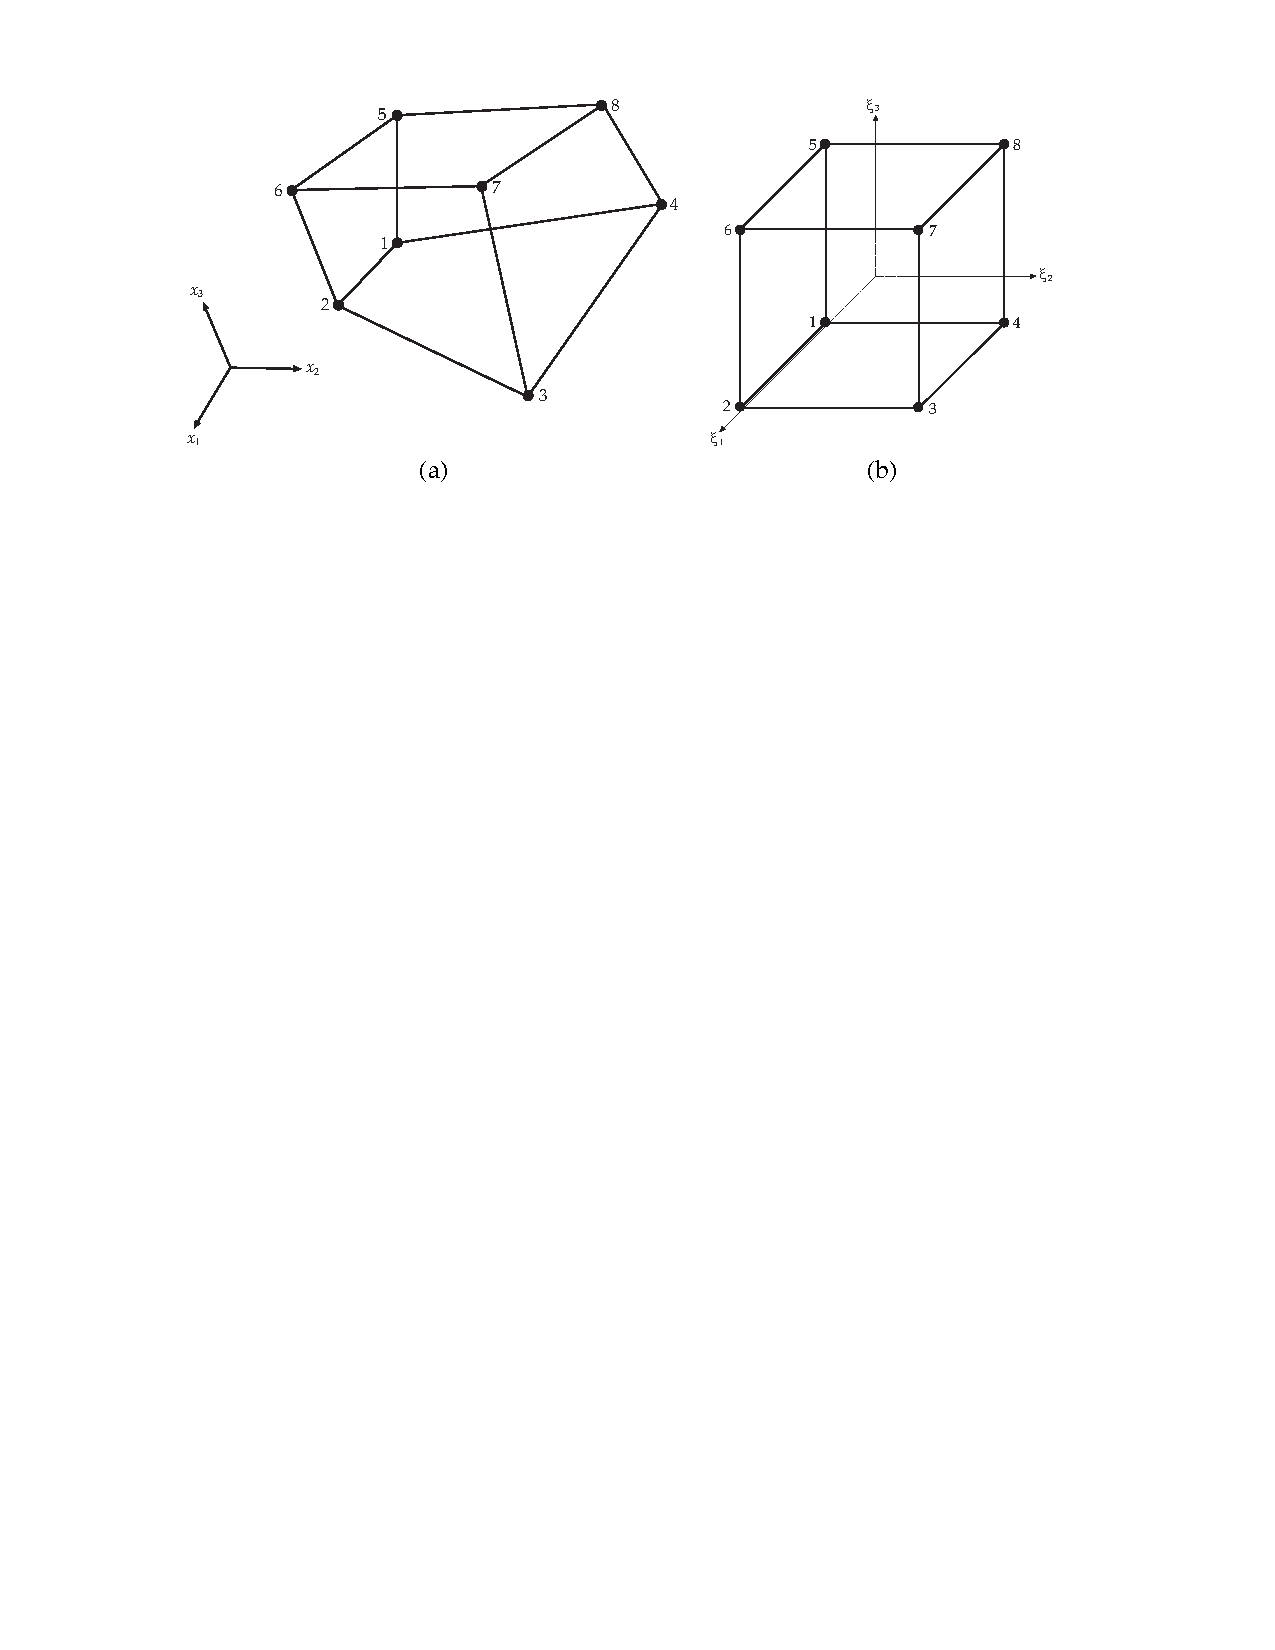
\includegraphics[width=13cm]{chapter3/naturalCoordinatesHexa.pdf}
\end{center}
\caption[Natural coordinates of a hexaedron]{Hexahedral element as it appears in the global coordinate system (a) and its natural coordinate system (b).}
\label{chap3:fig-naturalCoordinatesHexa}
\end{figure}
%
\begin{figure}[h]
\begin{center}
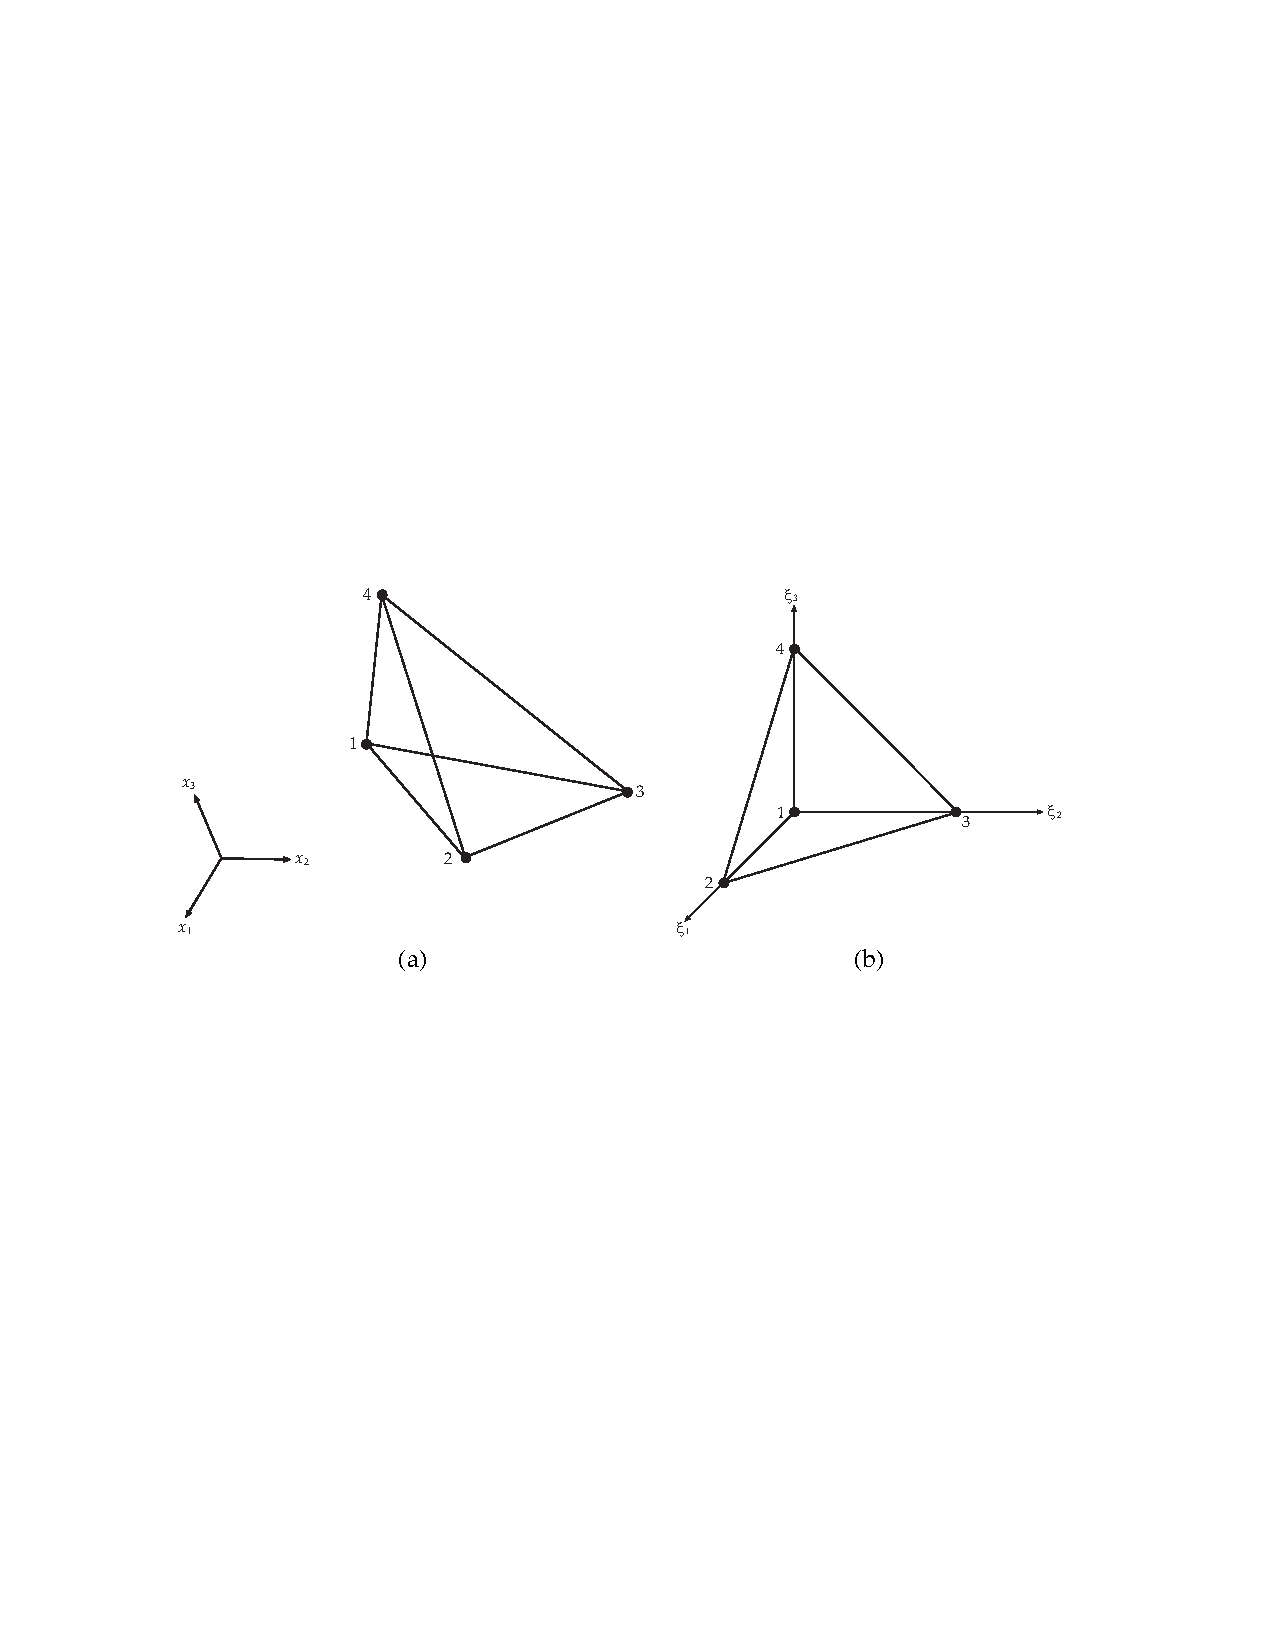
\includegraphics[width=13cm]{chapter3/naturalCoordinatesTetra.pdf}
\end{center}
\caption[Natural coordinates of a tetrahedron]{Tetrahedral element as it appears in the global coordinate system (a) and its natural coordinate system (b).}
\label{chap3:fig-naturalCoordinatesTetra}
\end{figure}

The use of the natural coordinate system has several advantages \citep{Biswas76}. Not only the interpolation functions can be derivated only once per type of element in the mesh, but their expression is also much simpler, regardless of the actual element shape. Consequently, the element equations and the derived element matrices get to be simplified too. However, we now need to switch between the natural and global coordinate systems before solving the equations on the whole domain. Indeed, it is necessary to account for the diversity of element shapes within the mesh. Solving the element equations expressed into the natural coordinate system would not yield the expected result for the whole domain. 
	
	
	\subsection{Geometry interpolation}
Let us assume a relation between the global coordinate $ x $ and the natural coordinate $ \xi $ in the following form:
\begin{equation}
\label{chap3:f}
x = f(\xi)
\end{equation}
where $ f $ is assumed to be a one-to-one correspondence (that is, a bijective function). This function may be seen as a transformation between the natural shape of the element and its arbitrary shape within the actual mesh, it describes a change in geometry. It is natural to think of approximating the geometry in a similar way that we approximated the solution in section \ref{chap3:solutionInterpolation}. Hence, the transformation defined by \eqref{chap3:f} may also be written as
\begin{equation}
\label{chap3:shapeFunctions}
x = \sum_{i=1}^m x_i^e \hat{\psi}_i^e(\xi)
\end{equation}
where $ x_i^e $ is the global coordinate of the $ i^{th} $ node of the element $ \Omega_e $, $ m $ the number of nodes for the element and $ \hat{\psi}_i^e(\xi) $ are the interpolation functions of degree $ m-1 $. Thus, we have a linear transformation when $ m = 2 $ and the relation betweeen $ x $ and $ \xi $ is quadratic when $ m=3 $. The interpolation functions $ \hat{\psi}_i^e(\xi) $ are called \emph{shape functions} because they are used to express the geometry or shape of the element. 
% Assuming the numbering of nodes in the global system follows the one of the natural system, the shape functions act as a mapping between the two representations. 

\bigskip

\noindent \textbf{Remark.}
It is worth noting that \eqref{chap3:shapeFunctions} can be easily extented to three-dimensional problems. Let us consider a Cartesian coordinate system and we denote the position of node $ i $ $ \mathbf{x}_i = [x_{i1}, x_{i2}, x_{i3}]^T$. The position of a point $ \mathbf{x} = [x_{1}, x_{2}, x_{3}]^T$ within the element may then be interpolated by applying \eqref{chap3:shapeFunctions} to each component of the position:
\begin{align}
x_1 &= \sum_{i=1}^m x_{i1} \hat{\psi}_i^e(\xi) \notag \\
x_2 &= \sum_{i=1}^m x_{i2} \hat{\psi}_i^e(\xi) \\
x_3 &= \sum_{i=1}^m x_{i3} \hat{\psi}_i^e(\xi) \notag
\end{align}
If we construct the vector $ \hat{\mathbf{x}}^e $ of all nodal positions $ \mathbf{x}_i $ of the element, we can define a shape function matrix $ \mathbf{H} $ such as:
\begin{equation}
\label{chap3:H}
\mathbf{x} = \mathbf{H} \hat{\mathbf{x}}^e
\end{equation}
where $ \mathbf{H} $ is a $ 3 \times m $ matrix built from submatrices $ \mathbf{H}_i $
\begin{equation}
\mathbf{H}_i = 
	\begin{bmatrix}
		\hat{\psi}_i^e & 0 & 0 \\
		0 & \hat{\psi}_i^e & 0 \\
		0 & 0 & \hat{\psi}_i^e
	\end{bmatrix}
\quad i = 1, 2, \ldots, m.
\end{equation}


	\subsection{A particular case: isoparametric elements}
% \noindent \textbf{Some remarks.}
Most of the time, we choose to interpolate the solution and the element geometry with the same interpolation functions. In this case, the elements are said to be \emph{isoparametric}. Under this configuration, natural coordinates appear as parameters that define the shape functions. Note that the shape functions describe the geometry and the solution with the same degree of interpolation. Because isoparametric elements are very common in practice, the use of the phrase \emph{shape functions} is often extented to denote the interpolation functions employed to approximate the solution.
	
	
\section{Derivation of element equations}	\label{chap3:derivationEquations}

Let us sum up where we are into the finite element analysis process so far. The whole domain has been divided into sub-domains, smaller, that we call elements, for which the solution to be sought will be simpler to find. We know how to approximate the solution within each of these elements using a linear combination of shape functions. And we even have a method to simplify the expression of these shape functions using natural coordinates. 

	\subsection{Strong and weak forms}
	
The next step is therefore to derive the element equations themselves. Obviously these equations depend on the type of problem that we seek to solve. From now on, we will only consider the context of continuum mechanics since our overall goal is the modelling of organ deformation. However, a similar approach can be used in the other fields of physics. In continuum mechanics, applying Newton's second law yields a partial differential system of equations. Such equations are called \emph{strong forms}. The strong form, in contrast to a \emph{weak form}, requires strong continuity on the dependent field variables, such as displacements \citep{Liu03}. The functions defining these field variables have to be differentiable up to the order of the partial differential equations that exist in the strong from. Obtaining the exact solution for a strong form is usually very difficult for practical engineering problems. We know that the finite element method can be used to find an approximated solution but the method usually works well only with regular geometry and boundary conditions.

A weak form is often created using energy principles or weighted residual methods. The weak form is often an integral form and requires a weaker continuity on the field variables. Due to the weaker requirement on the field variables, and the integral operation, a formulation based on a weak form usually produces a set of discretised system equations that give much more accurate results, especially for problems of complex geometry. Hence, the weak form is usually preferred for obtaining an approximate solution. Using the weak form usually leads to a set of well-behaved algebraic system equations, if the problem domain is discretised properly into elements.

	\subsection{Time dependence}
In all the equations of the finite element method that we derived so far, we have not taken time into account. For some problem, this is not an issue, the motion is sufficiently slow to assume that the dynamic effects (such as damping effect) are neglectable. However, this assumption is not always valid, particulary in our case where we want to model organ deformation. The deformation obviously depends on time. Finite element models of time-dependent problems can be developed in two alternatives ways \citep{Reddy93}:
\begin{description}
\item[(a)] coupled formulation in which the time $ t $ is treated as an additional coordinate along with the spatial coordinate $ x $
\item[(b)] decoupled formulation where time and spatial variations are assumed to be separable.
\end{description}
Thus, the approximation of the solution $ u $ takes one of these two forms:
\begin{align}
u(x, t) \approx u^e(x, t) &= \sum_{i=1}^n \hat{u}^e_i \hat{\psi}^e_i(x, t)  \quad \text{ (coupled formulation)} \label{chap3:approxTime1}\\
u(x, t) \approx u^e(x, t) &= \sum_{i=1}^n u^e_i(t) \psi^e_i(x) \quad \text{(decoupled formulation)} \label{chap3:approxTime2}
\end{align}
where $ \hat{\psi}^e_i(x, t) $ are time-space interpolation functions, $ \hat{u}^e_i $ are the nodal values that are independent of $ x $ and $ t $, $ \psi^e_i(x) $ are the usual interpolation functions in spatial coordinate $ x $ only and the nodal values $ u^e_i(t) $ are functions of time $ t $ only. Space-time coupled finite element formulations are not common and they have not been adequately studied. Hence, we consider the decoupled formulation only. Of course, the assumption that the time and spatial variations are separable is not valid in general. However, with sufficiently small time steps, it is possible to obtain accurate solutions nevertheless. 

	
	\subsection{Dynamic system of equations}	 \label{chap3:dynamic}
The space-time decoupled finite element formulation of time-dependent problems involves two steps:
\begin{description}
\item[1. Spatial approximation.]
The solution $ u $ is first approximated by expressions of the form \eqref{chap3:approxTime2} while keeping the time-dependent term during the finite element model derivation. This step leads to a set of ordinary differential equations in time.
\item[2. Temporal approximation.]
The system of ordinary differential equations is then approximated in time where different schemes may be used to assess the time derivatives. This step yields a set of algebraic equations for $ u^e_i $ at discrete time $ t_{k+1} = (k+1) \Delta t$ where $ \Delta t $ is the time increment and $ k > 0$ an integer. 
\end{description}
At the end of this two-step approximation, we have a continuous spatial solution at discrete intervals in time:
\begin{equation}
\label{chap3:approxTime}
u(x, t_k) \approx u^e(x, t_k) = \sum_{i=1}^n u^e_i(t_k) \psi^e_i(x) \quad \text{with } k = 0, 1, \ldots
\end{equation}
	
The construction of the weak form using either energy principles or weighted residual methods will not be detailed here. The reader may easily find it in dozens of textbooks. By substituting \eqref{chap3:approxTime} in the weak form, we obtain the finite element equations of equilibrium in matrix form:
\begin{equation}
\label{chap3:eqDynamic}
\mathbf{M}^e \mathbf{\ddot U}^e + \mathbf{D}^e \mathbf{ \dot U}^e + \mathbf{K}^e(\mathbf{U}^e) \cdot \mathbf{U}^e = \mathbf{R}^e,
\end{equation}
where $ \mathbf{M}^e $ is a constant mass matrix, $\mathbf{D}^e$ is a constant damping matrix, $ \mathbf{K}^e(\mathbf{U}^e) $ is the stiffness matrix, which is a function of nodal displacements $\mathbf{U}^e$, and $\mathbf{R}^e$ are externally applied loads. All matrices are expressed at the level of individual elements (which is the reason for the superscript $ ^e $).


	\subsection{Static system of equations}	\label{chap3:static}
Under some assumption, \eqref{chap3:eqDynamic} may be simplified. For instance, let us consider the problem of finding the maximum load that a desk can sustain. It is fair to say that strain and stress within the structure does not fluctuate over time: the system is in an equilibrium state. At all times, the sum of all forces applied on the system is equal to zero. Therefore, we can assume that the equations describing the structure do not depend on time: the problem is said to be \emph{static}. Static analyses assume that loading of a body occurs slowly enough that inertial and damping terms may be neglected. In this case, the static system of equations can be easily obtained by merely dropping out the dynamics terms in \eqref{chap3:eqDynamic}. Indeed, the static case may just be seen as a special case of the dynamic equations and the static equations are:
\begin{equation}
\label{chap3:eqStatic}
\mathbf{K}^e (\mathbf{U}^e ) \cdot \mathbf{U}^e  = \mathbf{R}^e .
\end{equation}

	\subsection{A few words on the matrices involved} \label{chap3:wordOnMatrices}
		
		\subsubsection*{Mass matrix}
The mass matrix $ \mathbf{M} $ for the whole domain may be computed by summing the mass contributions from every elements:
\begin{equation}
\mathbf{M} = \sum_e \mathbf{M}^e,
\end{equation}
where $ \mathbf{M}^e $ is the mass of element $ \Omega_e $ given by:
\begin{equation}
\mathbf{M}^e = \int_{V^e} \rho^e \mathbf{H}^T \mathbf{H} dV
\end{equation}
where $ \rho $ the mass density, $ V^e $ the volume of the element and $ \mathbf{H} $ is the shape function matrix defined by \eqref{chap3:H}. This integral may be evaluated using a procedure of numerical integration and generally results in a band mass matrix (non-zero entries are confined to a diagonal band, comprising the main diagonal and more diagonals on either side). This method for computing the mass matrix is called \emph{variational mass lumping}.

However, it is very common in finite element analysis to use a diagonal mass matrix. The most common way of achieving this is to define the diagonal entries with the sum of the corresponding rows and then set all other values to 0. The physical interpretation of this is lumping all of the mass in the volume surrounding a node at the node itself. A diagonal mass matrix may offer significant computational and storage advantages. First, it is easily inverted, since the inverse of a diagonal matrix is also diagonal. And a diagonal mass matrix can also be stored simply as a vector. Therefore, such a matrix may be built by directly computing the mass of each element and assigning an equal proportion of this to each of the element's nodes. This method is named \emph{direct mass lumping}. The mass $ m^e $ of element $ \Omega_e $ is given by:
\begin{equation}
m^e = \rho^e \int_{V^e} dV,
\end{equation}
which is integrated over the element using a numerical method. Each diagonal component of the mass matrix then receives a contribution of $ m^e/m $. 
		
		\subsubsection*{Damping matrix}
In a similar way to the mass matrix, a damping matrix may be defined by summing the damping contributions from every elements:
\begin{equation}
\mathbf{D} = \sum_e \mathbf{D}^e,
\end{equation}
where $ \mathbf{D}^e $ is the damping of element $ \Omega_e $ given by:
\begin{equation}
\mathbf{D}^e = \int_{V^e} \kappa^e \mathbf{H}^T \mathbf{H} dV
\end{equation}
where $ \kappa^e $ is a damping parameter. In practice, the components of damping matrices are difficult to determine experimentally. Therefore, it is common to employ the \emph{Rayleigh damping}. The Rayleigh damping assumes that the damping may be written in the form of:
\begin{equation}
\mathbf{D}^e = \alpha \mathbf{M}^e + \beta \mathbf{K}^e,
\end{equation}
where $ \alpha $ and $ \beta $ are coefficients defining mass and stiffness proportional damping components. However, for systems with large degrees of freedom, it is difficult to guess meaningful values of $ \alpha $ and $ \beta $. \cite{Chowdhury03} have proposed a method to calculate these coefficients. In practice, further assumptions may only lead to include the mass proportional component ($ \beta = 0 $), which yields a diagonal damping matrix if a diagonal mass matrix is used. 

		
		\subsubsection*{Stiffness matrix}
The expression of the stiffness matrix depends on the chosen strain tensor as well as the appropriate constitutive model for the material. Its general form cannot be explicited. However, it can be demonstrated that $ \mathbf{K}^e $ may be written as
\begin{equation}
\mathbf{K}^e = \int_{V^e} \mathbf{B}^T \mathbf{E} \, \mathbf{B} \, dV,
\end{equation}
where $ \mathbf{E} $ is a material matrix, which only depends on the constitutive model chosen, and $ \mathbf{B} $ is the \emph{strain-displacement matrix} defined as the derivatives of the shape functions (see \cite{Liu03,Belytschko00} for details). 
	
	

\section{Assembly of element equations}
We have now derived the equations for each element. However, since the element is physically connected to its neighbours, the resulting algebraic equations will contain more unknowns than the number of algebraic equations. In other words, elements share vertices. The deformation of an element induces the deformation of its neighbours. Thus, it becomes necessary to put the elements together to eliminate the extra unknowns, to model this interaction between elements. The assembly of the global stiffness matrix should be carried out as soon as the element matrices are computed, rather than waiting until the element coefficients of all elements are computed. This would require storage of the coefficients for each element. Instead, we can perform the assembly while we calculate the element matrices.  

The assembly operation is actually quite simple. Let us consider an example with stiffness matrices for an one-dimensional problem. We assume that we have three two-node elements. And we suppose the element connectivity information given by Table \ref{chap3:connectivity}, which provides the global node number for each local node number within an element. 
\begin{table}
	\begin{center}
	\begin{tabular}{|c|c|c|}
		\hline Elements & 1 & 2 \\ 
		\hline 1 & 1 & 2 \\ 
		\hline 2 & 2 & 3 \\ 
		\hline 3 & 3 & 4 \\ 
		\hline 
		\end{tabular} \caption{Element connectivity information}
		\label{chap3:connectivity}
	\end{center}
\end{table}
We also assume the following stiffness matrices for the three elements:
\begin{equation}
\mathbf{K}^1 = 
\color{blue}
	\begin{bmatrix}
	-1 & 2 \\
	3 & 1
	\end{bmatrix}
\color{black}
\text{, } \quad 
\mathbf{K}^2 = 
\color{green}
	\begin{bmatrix}
	5 & 2 \\
	-2 & 1
	\end{bmatrix}
\color{black}
\text{ and } \quad 
\mathbf{K}^3 = 
\color{red}
	\begin{bmatrix}
	3 & 1 \\
	2 & -1
	\end{bmatrix}
\color{black}
\end{equation}
The assembled matrix is a square matrix of dimension number of nodes $\times$ number of degrees of freedom. In our case, the global matrix is therefore a $ 4 \times 4 $ and is assembled in the following manner:
\begin{equation}
\mathbf{K} = 
	\begin{bmatrix}
	\color{blue}{-1} & \color{blue}{2} & \color{black}{0} & 0 \\
	\color{blue}{3} & \color{blue}{1}\color{black}{+}\color{green}{5} & \color{green}{2} & \color{black}{0} \\
	0 & \color{green}{-2} & \color{green}{1} \color{black}{+} \color{red}{3} & \color{red}{1} \\
	\color{black}{0} & 0 & \color{red}{2} & \color{red}{-1}
	\end{bmatrix}
\color{black}
\end{equation}
In other words, the global matrix is merely a rewritting on the whole domain of the element stiffness matrices, which are expressed with respect to local node numbers, in terms of global node numbers. In addition to constructing the global mass and damping matrices (as shown in section \ref{chap3:wordOnMatrices}), this process leads to the following global system of equations:
\begin{equation}
\label{chap3:dynamic2}
\mathbf{M} \mathbf{\ddot U} + \mathbf{D} \mathbf{ \dot U} + \mathbf{K}(\mathbf{U}) \cdot \mathbf{U} = \mathbf{R}.
\end{equation}	
The same set of equations was established at the element level in section \ref{chap3:dynamic} but we may note that the same system is also valid for the whole domain. 


\section{Solution of global problem}
The complete and global system of equations has now been established. In this section, we will examine the techniques commonly used for solving these equations. In the general case of a dynamic system of equations, the equations are not yet algebraic and still depends on derivatives of the unknown displacements with respect to time. Therefore, an additional step needs to be performed before using a solver by integrating the equations over time. As we will see shortly, the different methods of time integration are classified into two main schemes: \emph{explicit} or \emph{implicit} integration. We begin by introducing the simplest method, the Euler method to explain the concept of an explicit method. Then the central difference method will be detailled. We then describe a few implicit methods, allowing us to highlight the relative advantages of the two types of methods. Finally, the static case will be solved by emphasizing the similarities with implicit systems through the critical step of linearisation of the governing equations \citep{Belytschko00}.

	\subsection{Explicit time integration}

		\subsubsection*{The Euler method}	
We want to approximate the solution of the following differential equation:
\begin{equation}
\label{chap3:eqToSolve}
\mathbf{\dot U}^t = f(t, \mathbf{U}^t).
\end{equation}
Note that we restrict ourselves to first-order differential equations (meaning that only the first derivative of $\mathbf{U}^t$ appears in the equation, and no higher derivatives). However, a higher-order equation can easily be converted to a system of first-order equations by introducing extra variables. For example, the second-order equation $\mathbf{\ddot U}^t = -\mathbf{U}^t$ can be rewritten as two first-order equations: $\mathbf{\dot U}^t = \mathbf{V}^t$ and $\mathbf{\dot V}^t = -\mathbf{U}^t$. By solving equations like \eqref{chap3:eqToSolve}, we will therefore be able to integrate the global system of equations over time. 

We start by replacing the derivative $\mathbf{\dot U}^t $ by the finite difference approximation:
\begin{equation}
\label{chap3:approxExplicit}
\mathbf{\dot U}^t \approx \dfrac{\mathbf{U}^{t+\Delta t} - \mathbf{U}^t}{\Delta t},
\end{equation}
which gives:
\begin{equation}
\mathbf{U}^{t+\Delta t} \approx \mathbf{U}^t + \Delta t \, \mathbf{\dot U}^t
\end{equation}
And substituting the last relation in \eqref{chap3:eqToSolve} yields:
\begin{equation}
\label{chap3:updateExplicit}
\mathbf{U}^{t+\Delta t} \approx \mathbf{U}^t + \Delta t \, f(t, \mathbf{U}^t)
\end{equation}
This formula is usually applied in a recursive scheme. We choose a time step $ \Delta t $ and we construct the sequence of time $ t^n = n \Delta t$. Using \eqref{chap3:updateExplicit}, we can approximate the exact solution $ \mathbf{U}^{t^n} $ at each time step by $ \mathbf{U}^n $:
\begin{equation}
\mathbf{U}^{n+1} = \mathbf{U}^n + \Delta t \, f(t^n, \mathbf{U}^n).
\end{equation}
This method is called \emph{Euler method} and is said to be explicit because the new value $ \mathbf{U}^{n+1} $ is defined in terms of variables from the previous time step $ \mathbf{U}^n $.


		\subsubsection*{The central difference method}	
The central difference method is one of the most popular explicit methods in computational mechanics. This method is based on central difference formulas for the velocity and acceleration. Let us the time $ t $ of the simulation be subdivided into time steps $ \Delta t $. Let us denote by $ \mathbf{U}^t $, $ \mathbf{\dot U}^t $ and $ \mathbf{\ddot U }^t $ the matrices of nodal displacements, velocities and accelerations, respectively, at time $ t $. The central difference method makes use of the following finite differences approximations for acceleration and velocity:
\begin{align}
\mathbf{\ddot U}^t &= \dfrac{1}{(\Delta t)^2} \left( \mathbf{U}^{t-\Delta t} - 2 \mathbf{U}^{t} +\mathbf{U}^{t+\Delta t} \right) \label{chap3:accelerationApprox}\\
\mathbf{\dot U}^t &= \dfrac{1}{2 \Delta t} \left( \mathbf{U}^{t+\Delta t} - \mathbf{U}^{t-\Delta t} \right). \label{chap3:velocityApprox}
\end{align}
One of the key advantage of the method is that the stifness term in \eqref{chap3:dynamic2} may be computed from
\begin{equation}
\mathbf{K}(\mathbf{U}) \cdot \mathbf{U} = \mathbf{F}(\mathbf{U}) = \sum_e \tilde{\mathbf{F}}^e,
\end{equation}
where $ \tilde{\mathbf{F}}^e $ are the global nodal force contributions due to stresses in element $ \Omega_e $. $ \tilde{\mathbf{F}} $ may be computed using strain-displacement equations, the constitutive equation and the element connectivity. Therefore, let us assume that all nodal forces $\mathbf{F}^t $  at time $ t $ are known. 

By subtituting \eqref{chap3:accelerationApprox} and \eqref{chap3:velocityApprox} into \eqref{chap3:dynamic2} we obtain:
\begin{equation}
\left( \dfrac{\mathbf{M}}{(\Delta t)^2} + \dfrac{\mathbf{D}}{2 \Delta t} \right) \mathbf{U}^{t+\Delta t} = \mathbf{R}^t - \mathbf{F}^t + \dfrac{2 \mathbf{M}}{(\Delta t)^2} \mathbf{U}^t + \left( \dfrac{\mathbf{D}}{2 \Delta t} - \dfrac{\mathbf{M}}{(\Delta t)^2} \right) \mathbf{U}^{t-\Delta t}.
\end{equation}
Both the right-hand side of the equation and the factor in front $ \mathbf{U}^{t+\Delta t} $ may be evaluated, which gives the nodal displacements for the next time step. The entire update can be accomplished without solving any system of equations provided that the mass matrix $ \mathbf{M} $ and the damping matrix $ \mathbf{D} $ are diagonal. As we have seen in section \ref{chap3:wordOnMatrices}, these approximations are often used in practice. And this is the characteristic of an explicit method: the time integration of the general system of equations for finite element model does not require the solution of any equations. This is a key point because it gives explicit methods a tremendous computational advantage. However, explicit methods are only conditionally stable. If the time step exceeds a critical value, the solution may be erroneous. This critical time step depends on the mesh and the material properties. It will decrease with mesh refinement and increasing stiffness of the material. 


%\begin{equation}
%\label{chap3:diffV}
%\mathbf{V} ^{n+\frac{1}{2}} = \dfrac{1}{\Delta t^{n+\frac{1}{2}}} \left(\mathbf{U} ^{n+1} - \mathbf{U} ^{n} \right).
%\end{equation}
%By rearranging \eqref{chap3:diffV}, we may obtain:
%\begin{equation}
%\mathbf{U} ^{n+1} = \mathbf{U} ^{n} + \Delta t^{n+\frac{1}{2}} \mathbf{V}^{n+\frac{1}{2}}
%\end{equation}
%The acceleration is given by:
%\begin{align}
%\label{chap3:diffA}
%\mathbf{A} ^{n} &= \dfrac{1}{ \Delta t^{n}} \left(\mathbf{V}^{n+\frac{1}{2}} - \mathbf{V}^{n-\frac{1}{2}} \right), \\
%\mathbf{V} ^{n+\frac{1}{2}} &= \mathbf{V}^{n-\frac{1}{2}} + \Delta t^{n} \mathbf{A}^{n}.
%\end{align}
%By substituting \eqref{chap3:diffV} and its counterpart for the previous time step into \eqref{chap3:diffA}, the acceleration can be expressed directly in terms of the displacements:
%\begin{equation}
%\mathbf{A}^n = \dfrac{ \Delta t^{n-\frac{1}{2}} \left( \mathbf{U}^{n+1} - \mathbf{U}^{n} \right) - \Delta t^{n+\frac{1}{2}} \left( \mathbf{U}^{n} - \mathbf{U}^{n-1} \right) }{ \Delta t^{n} \Delta t^{n-\frac{1}{2}} \Delta t^{n+\frac{1}{2}} }
%\end{equation}
%If the time steps are all equals, the latter expression can be reduced to:
%\begin{equation}
%\mathbf{A}^n = \dfrac{ \left( \mathbf{U}^{n+1} -2 \mathbf{U}^{n} + \mathbf{U}^{n-1} \right) }{ \left( \Delta t^n \right)^2 }.
%\end{equation}
%This is the well-known formula for the second derivative of a function. 

%We now consider the time integration of the dynamic system of equations. Equations \eqref{chap3:dynamic2} may be written as:
%\begin{equation}
%\mathbf{M} \mathbf{A}^n = \mathbf{F}_{\text{ext}}(\mathbf{U}, t^n) - \mathbf{F}_{\text{int}}(\mathbf{U}, \mathbf{V}, t^n).
%\end{equation}
%where $ \mathbf{F}_{\text{int}} $ and $ \mathbf{F}_{\text{ext}} $ are the internal and external forces, respectively. The external loads are usually provided as functions of time and they may depends on nodal displacements (as when a pressure is applied). The internal forces depend on displacements and velocities through the stiffness and damping matrices. 

	\subsection{Implicit time integration}
	
		\subsubsection*{The backward Euler method}
The problem that we wish to solve is the same than the one we introduced with the Euler method, which we reproduce here for convenience:
\begin{equation}
\mathbf{\dot U}^t = f(t, \mathbf{U}^t).
\end{equation}
This time, instead of using \eqref{chap3:approxExplicit}, we approximate the derivative $ \mathbf{\dot U}^t $ by:
\begin{equation}
\mathbf{\dot U}^t \approx \dfrac{\mathbf{U}^t - \mathbf{U}^{t-\Delta t}}{\Delta t}.
\end{equation}
The update expression for $ y^n $ then becomes:
\begin{equation}
\mathbf{U}^{n+1} = \mathbf{U}^n + \Delta t \, f(t^{n+1}, \mathbf{U}^{n+1}).
\end{equation}
The \emph{backward Euler method} is an implicit method, meaning that we have to solve an equation to find $ \mathbf{U}^{n+1} $. Of course, it costs time to solve this equation and this cost must be taken into consideration when we select the time integration method to use. The advantage of implicit methods is that they are usually more stable for solving a stiff equation, meaning that larger steps can be used. 

	\subsubsection*{The Runge-Kutta method}
The accuracy of backward Euler method can be improved by making the solution depends on more values. The $ 4^{th} $ order Runge-Kutta method gives the following update equation:
\begin{equation}
\mathbf{U}^{n+1} = \mathbf{U}^{n} + \frac{1}{6} \Delta t \left( k_1 + 2 k_2 + 2 k_3 +k_4 \right),
\end{equation}
where :
\begin{align}
k_1 &= f(t^n, \mathbf{U}^n) \notag \\
k_2 &= f(t^n + \frac{1}{2} \Delta t, \mathbf{U}^n + \frac{1}{2} \Delta t \, k_1) \notag \\
k_3 &= f(t^n + \frac{1}{2} \Delta t, \mathbf{U}^n + \frac{1}{2} \Delta t \, k_2) \notag \\
k_4 &= f(t^n + \Delta t, \mathbf{U}^n + \Delta t \, k_3) \notag
\end{align}
This method is a fourth-order method because the total accumulated error has order $ \Delta t^4 $. It may be seen as a generalisation of the backward Euler method \citep{Press92}. Again, we have to solve an equation to find $ \mathbf{U}^{n+1} $. 

	\subsection{Static solutions}
First, we recall the general system of equations in static introduced in section \ref{chap3:static}, which is also valid for the whole system: 
\begin{equation}
\mathbf{K}(\mathbf{U}) \cdot \mathbf{U} = \mathbf{R}.
\end{equation}	
The situation is similar to implicit time integration methods for dynamic systems by the fact that we also have to solve a set of algebraic equations to find the nodal displacements. In the general case, the equations are non-linear and therefore quite difficult to solve. A suitable solver for this kind of system is, for instance, the \emph{Newton-Raphson} method. In essence, this method consists of obtaining linear equations instead. This process is called \emph{linearisation}. One may refer to \citep{Belytschko00} for more details. 

However, if the problem is linear, the stiffness matrix does not depend on the displacement and the resolution is facilitated. The unknown displacements may be computed by:
\begin{equation}
\mathbf{U} = \mathbf{K}^{-1} \, \mathbf{R}.
\end{equation}
Many techniques are available in the literature to solve this type of system, and a few of them are introduced in the next section. 



%	\subsection{Dynamic problems}
%Let us recall the general system of equations in dynamic introduced in section \ref{chap3:dynamic}, which is also valid for the whole system: 
%\begin{equation}
%\label{chap3:dynamic2}
%\mathbf{M} \mathbf{\ddot U} + \mathbf{U} \mathbf{ \dot U} + \mathbf{K}(\mathbf{U}) \cdot \mathbf{U} = \mathbf{R}.
%\end{equation}	
%In the general case of a dynamic system of equations, the equations are not yet algebraic and still depends on derivatives of the unknown displacements with respect to time. Therefore, an additional step needs to be performed before using a solver by integrating the equations over time. The different methods of time integration are classified into two main schemes: \emph{explicit} or \emph{implicit} integration. If positions and velocities are extrapolated from their values obtained at the previous time step, then this approach is qualified of explicit. Conversely, if positions and velocities are considered as unknowns for the current time step, the scheme is called implicit. The choice of one scheme over the other impacts the stability and the computational time. 
%
%		\subsubsection*{Explicit time integration}
%Explicit schemes make use	 of data from the previous time step to assess the ones from current time step. From \eqref{chap3:dynamic2} we have:
%\begin{align}
%\mathbf{M} \mathbf{\ddot U} &= \mathbf{R} - (\mathbf{U} \mathbf{ \dot U} + \mathbf{K}(\mathbf{U}) \cdot \mathbf{U}) \notag \\
%\mathbf{M} \mathbf{\ddot U} &= \mathbf{F}_{\textbf{ext}} - \mathbf{F}_{\textbf{int}}(\mathbf{U}, \mathbf{\dot U})
%\end{align}
%where $ \mathbf{F}_{\textbf{int}} $ and $ \mathbf{F}_{\textbf{ext}} $ are the internal and external forces, respectively. We denote $ \mathbf{U}_i - \mathbf{U}_{i-1} = \Delta U = h \mathbf{\dot U}_{i-1} $ and $ \mathbf{\dot U}_i - \mathbf{\dot U}_{i-1} = \Delta \dot U = h \mathbf{\ddot U}_{i-1} $ and we may write:
%\begin{equation}
%	\begin{pmatrix}
%		\Delta U \\
%		\Delta \dot U
%	\end{pmatrix}
%	= 
%	h 
%	\begin{pmatrix}
%		\mathbf{\dot U}_{i-1} \\
%		\mathbf{M}^{-1} \, (\mathbf{F}_{\textbf{ext}} - \mathbf{F}_{\textbf{int}}(\mathbf{U}, \mathbf{\dot U}))
%	\end{pmatrix}
%\end{equation}
%We note that this scheme does not require any resolution of system if the mass matrix was diagonalised by mass lumping as explained in section \ref{chap3:massMatrix}. It is therefore a particulary efficient algorithm. However, this kind of scheme is only conditionally stable and requires small time steps. Thus, the gain in computation must be balanced against the need to calculating more steps. This lack of stability increases with smaller elements and stiffer materials. 

		
	\subsection{Solvers}	\label{chap3:solvers}
We will now examine the techniques commonly used for solving linear systems of algebraic equations. Note that this is only the most classical approaches and the list is obviously not exhaustive. Two categories of techniques are in opposition: \emph{direct} or \emph{iterative} solvers \citep{Press02}. In any case, we seek the solution for the unknown solution $ \mathbf{x}$ of the following system of linear equations:
\begin{equation}
\label{chap3:linearEquation}
\mathbf{A} \mathbf{x} = \mathbf{b}.
\end{equation}
The system may already be linear by nature, or been linearised using techniques such as Newton-Raphson methods. At this point in the discussion, we are therefore only interested in solving a linear system of equations. If the matrix $ \mathbf{A} $ is squared, which is the case in finite element methods, the problem may be written as follows:
\begin{equation}
\mathbf{x} = \mathbf{A}^{-1} \, \mathbf{b}.
\end{equation}

However, only solvers relevant to the context of finite element methods will be discussed. Indeed the matrix $ \mathbf{A} $ takes a specific form in problems solved by finite element methods. The matrix $ \mathbf{A} $ is \emph{sparse}. A sparse matrix is merely a matrix populated mainly with zeros. An example is given by \fig{chap3:fig-sparse} for a finite element problem in two dimensions.
\begin{figure}
\begin{center}
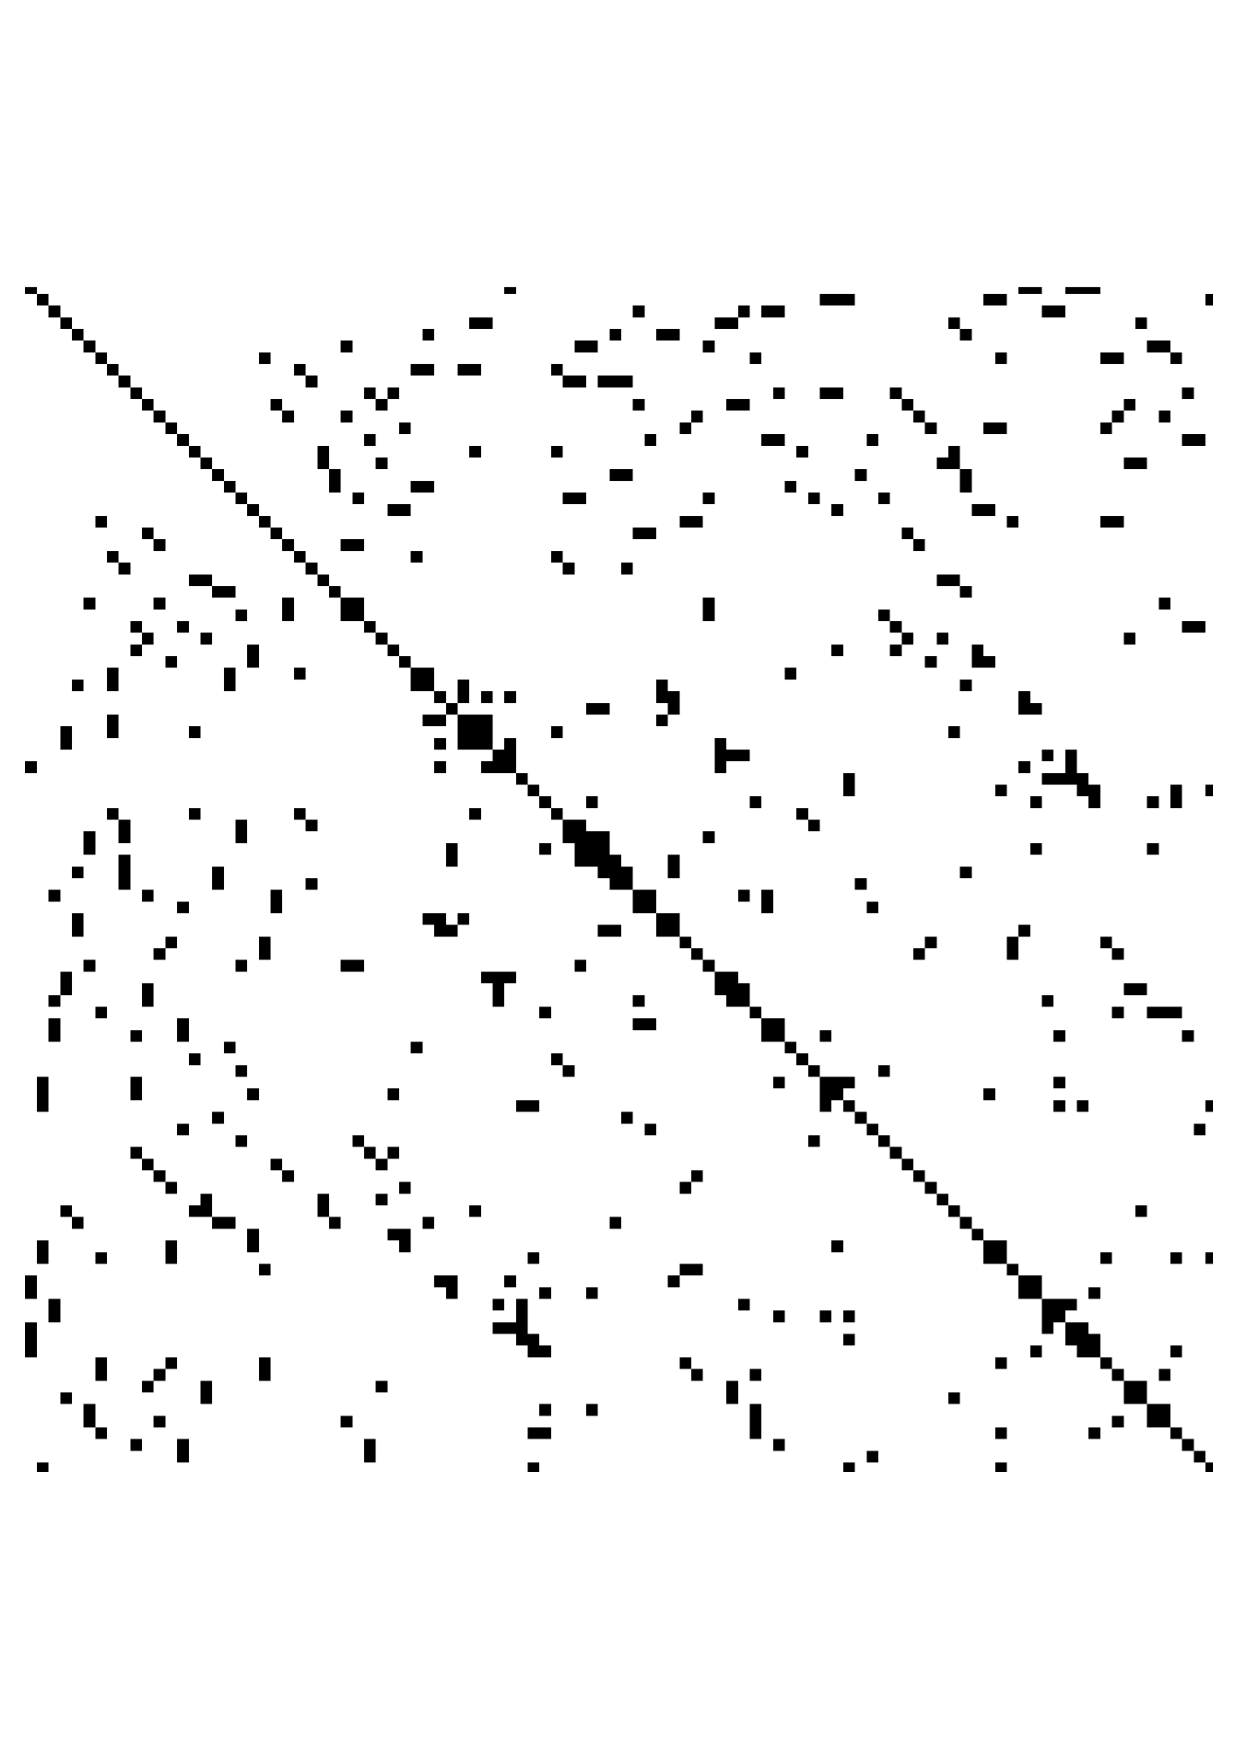
\includegraphics[width=13cm]{chapter3/sparse_matrix.pdf}
\end{center}
\caption[Illustration of a sparse matrix for a 2D finite element problem]{Illustration of a sparse matrix for a two-dimensional finite element problem. Each non-zero elements of the matrix is represented in black. Image courtesy of Oleg Alexandrov.}
\label{chap3:fig-sparse}
\end{figure}
Because of the peculiar structure of the matrix involved in finite element computations, methods have been specifically designed to take advantage of this structure. Indeed, it is wasteful to use general methods of linear algebra on such problems, because most of the arithmetic operations devoted to solving the set of equations or inverting the matrix involve zero operands. Furthermore, it is wasteful to reserve storage for zero elements. 

%The choice of a resolution method depends on the problem (linear or non-linear) and the properties of the stiffness matrix.
	
		\subsubsection*{Direct solvers}
As their name is suggesting, direct solvers make an attempt into finding a solution directly by inverting the matrix $ \mathbf{A} $. They execute in a predictable number of operations. We will now introduce a few direct methods in the context of finite element methods. 
% Methods such as Gauss-Jordan elimination or LU decomposition will not be discussed in this section for instance for their lack of efficiency with sparse matrices.

\paragraph*{LU decomposition.}
The LU decomposition is a matrix decomposition which writes a matrix as the product of a lower triangular matrix and an upper triangular matrix. In other words, $ \mathbf{A} $ may be written as:
\begin{equation}
\label{chap3:LU}
\mathbf{A} = \mathbf{L} \mathbf{U},
\end{equation}
where $ \mathbf{L} $ is lower triangular (has elements only on the diagonal and below) and $ \mathbf{U} $ is upper triangular (has elements only on the diagonal and above). As an example, for the case of a $ 4 \times 4 $ matrix $ \mathbf{A} $, we have:
\begin{equation}
	\begin{bmatrix}
	a_{11} & a_{12} & a_{13} & a_{14} \\
	a_{21} & a_{22} & a_{23} & a_{24} \\
	a_{31} & a_{32} & a_{33} & a_{34} \\
	a_{41} & a_{42} & a_{43} & a_{44}
	\end{bmatrix}
=
	\begin{bmatrix}
	\alpha_{11} & 0 & 0 & 0 \\
	\alpha_{21} & \alpha_{22} & 0 & 0 \\
	\alpha_{31} & \alpha_{32} & \alpha_{33} & 0 \\
	\alpha_{41} & \alpha_{42} & \alpha_{43} & \alpha_{44}
	\end{bmatrix}
	\begin{bmatrix}
	\beta_{11} & \beta_{12} & \beta_{13} & \beta_{14} \\
	0 & \beta_{22} & \beta_{23} & \beta_{24} \\
	0 & 0 & \beta_{33} & \beta_{34} \\
	0 & 0 & 0 & \beta_{44}
	\end{bmatrix}
\end{equation}
By subtituting \eqref{chap3:LU} into \eqref{chap3:linearEquation} we obtain:
\begin{equation}
\mathbf{A} \mathbf{x} = (\mathbf{L} \mathbf{U}) \mathbf{x} = \mathbf{L} (\mathbf{U} \mathbf{x}) = \mathbf{b}.
\end{equation}
Therefore, we can solve \eqref{chap3:linearEquation} by first solving the vector $ \mathbf{y} $ such that:
\begin{equation}
\label{chap3:eqLyb}
\mathbf{L} \mathbf{y} = \mathbf{b}
\end{equation}
and then solving 
\begin{equation}
\label{chap3:eqUxy}
\mathbf{U} \mathbf{x} = \mathbf{y}.
\end{equation}
The advantage of breaking up one linear set of equations into two successive ones is that the solution of a triangular set of equations is quite trivial. Indeed, \eqref{chap3:eqLyb} can be solved by:
\begin{equation} 
\left\lbrace
	\begin{aligned}
		y_1 &= \dfrac{b_1}{\alpha_{11}}  \\	
		y_i &= \dfrac{1}{\alpha_{ii}} \left[ b_i - \sum_{j=1}^{i-1} \alpha_{ij} y_j \right] \quad i = 2, 3, \ldots, N.
	\end{aligned} 
\right.
\end{equation}
for a $ N \times N $ matrix $ \mathbf{A} $. We then solve \eqref{chap3:eqUxy} in a similar way:
\begin{equation} 
\left\lbrace
	\begin{aligned}
		x_N &= \dfrac{y_N}{\beta_{NN}} \\	
		x_i &= \dfrac{1}{\beta_{ii}} \left[ y_i - \sum_{j=i+1}^{N} \beta_{ij} x_j \right] \quad i = N-1, N-2, \ldots, 1. 
	\end{aligned} 
\right.
\end{equation}


		\subsubsection*{Iterative solvers}
An iterative method attempts to solve the system of equations by finding successive approximations to the solution starting from an initial guess. In the case of a system of linear equations, the two main classes of iterative methods are the stationary iterative methods, and the more general Krylov subspace methods. Stationary iterative methods solve a linear system with an operator approximating the original one and based on a measurement of the error in the result (called the residual), form an equation of correction for which this process is repeated. While these methods are simple to derive, convergence is only guaranteed for a limited class of matrices. Examples of stationary iterative methods are the Jacobi method and Gauss-Seidel method. Krylov subspace methods work by forming an orthogonal basis of the sequence of successive matrix powers times the initial residual (the Krylov sequence). The approximations to the solution are then formed by minimising the residual over the subspace formed. The typical method in this class is the conjugate gradient method (CG). 
In practice, for large system of equations (as often encountered in finite element analysis), direct methods would take too much time and an iterative solvers is commonly used. 

\paragraph*{The Gauss-Seidel method.}
For this method, convergence is only guaranteed if the matrix is either diagonally dominant, or symmetric and positive-definite. In a similar way than the LU decomposition, we start by decomposing the matrix $ \mathbf{A} $ into a lower triangular component $ \mathbf{L}_ {*} $ and a strictly upper triangular component $ \mathbf{U} $:
\begin{equation}
\mathbf{A} = \mathbf{L}_{*} + \mathbf{U}.
\end{equation}
The system of linear equations \eqref{chap3:linearEquation} may be rewritten as:
\begin{equation}
\mathbf{L}_{*} \mathbf{x} = \mathbf{b} - \mathbf{U} \mathbf{x}
\end{equation}
The Gauss-Seidel method is an iterative technique that solves the left-hand side of the expression for $ \mathbf{x} $ using previous values for $ \mathbf{x} $ on the right-hand side. That is:
\begin{equation}
\mathbf{x}^{n+1} = \mathbf{L}_{*}^{-1} (\mathbf{b} - \mathbf{U} \mathbf{x}^n).
\end{equation}
Similarly to the LU decomposition method, we take advantage of the triangular form of $ \mathbf{L}_{*} $. The components of $ \mathbf{x}^{n+1} $ can be computed sequentially in the following manner:
\begin{equation}
x_i^{n+1} = \dfrac{1}{a_{ii}} \left[ b_i - \sum_{j>i} a_{ij} x_j^n -\sum_{j<i} a_{ij} x_j^{n+1} \right] \quad i = 1, 2, \ldots, N.
\end{equation}
The procedure is usually continued until the changes made by an interation are below a given threshold. 

\paragraph*{The conjugate gradient method.}		
The simplest class of conjugate gradient method is based on the idea of minimising the quadratic function:
\begin{equation}
f(\mathbf{x}) = \frac{1}{2} \mathbf{x}^T \, \mathbf{A} \, \mathbf{x} - b^T \, \mathbf{x} + c.
\end{equation}
Indeed, if the matrix $ \mathbf{A} $ is symmetric and positive-definite, $ f(\mathbf{x}) $ is minimised by the solution to $ \mathbf{A} \mathbf{x} = \mathbf{b} $ \citep{Shewchuk94}. The minimisation is carried out by generating a succession of search directions $ \mathbf{p} _k $ and improved minimisers $ \mathbf{x} _k $. At each stage a quantity $ \alpha_k $ is found that minimises $f(\mathbf{x}_k  + \alpha_k \mathbf{p}_k)$, and $\mathbf{x}_{k+1}$ is set equal to the new point $\mathbf{x}_k + \alpha_k \mathbf{p}_k$. The $ \mathbf{p}_k $  and $ \mathbf{x}_k $  are built up in such a way that $ \mathbf{x}_{k+1} $  is also the minimiser of $ f $ over the whole vector space of directions already taken, that is the space formed by the basis of vector ${\mathbf{p}_1, \mathbf{p}_2, \ldots, \mathbf{p}_k }$. After $N$ iterations, you arrive at the minimiser over the entire vector space, that is, the solution to our linear system of equations. 

Later, the \emph{biconjugate gradient method} was introduced as a generalisation of the ordinary conjugate gradient to solve systems where the matrix $ \mathbf{A} $ was not necessarily symmetric and positive-definite (see \cite{Belytschko00} for details). 	